% Options for packages loaded elsewhere
\PassOptionsToPackage{unicode}{hyperref}
\PassOptionsToPackage{hyphens}{url}
%
\documentclass[
]{article}
\usepackage{amsmath,amssymb}
\usepackage{iftex}
\ifPDFTeX
  \usepackage[T1]{fontenc}
  \usepackage[utf8]{inputenc}
  \usepackage{textcomp} % provide euro and other symbols
\else % if luatex or xetex
  \usepackage{unicode-math} % this also loads fontspec
  \defaultfontfeatures{Scale=MatchLowercase}
  \defaultfontfeatures[\rmfamily]{Ligatures=TeX,Scale=1}
\fi
\usepackage{lmodern}
\ifPDFTeX\else
  % xetex/luatex font selection
\fi
% Use upquote if available, for straight quotes in verbatim environments
\IfFileExists{upquote.sty}{\usepackage{upquote}}{}
\IfFileExists{microtype.sty}{% use microtype if available
  \usepackage[]{microtype}
  \UseMicrotypeSet[protrusion]{basicmath} % disable protrusion for tt fonts
}{}
\makeatletter
\@ifundefined{KOMAClassName}{% if non-KOMA class
  \IfFileExists{parskip.sty}{%
    \usepackage{parskip}
  }{% else
    \setlength{\parindent}{0pt}
    \setlength{\parskip}{6pt plus 2pt minus 1pt}}
}{% if KOMA class
  \KOMAoptions{parskip=half}}
\makeatother
\usepackage{xcolor}
\usepackage[margin=1in]{geometry}
\usepackage{color}
\usepackage{fancyvrb}
\newcommand{\VerbBar}{|}
\newcommand{\VERB}{\Verb[commandchars=\\\{\}]}
\DefineVerbatimEnvironment{Highlighting}{Verbatim}{commandchars=\\\{\}}
% Add ',fontsize=\small' for more characters per line
\usepackage{framed}
\definecolor{shadecolor}{RGB}{248,248,248}
\newenvironment{Shaded}{\begin{snugshade}}{\end{snugshade}}
\newcommand{\AlertTok}[1]{\textcolor[rgb]{0.94,0.16,0.16}{#1}}
\newcommand{\AnnotationTok}[1]{\textcolor[rgb]{0.56,0.35,0.01}{\textbf{\textit{#1}}}}
\newcommand{\AttributeTok}[1]{\textcolor[rgb]{0.13,0.29,0.53}{#1}}
\newcommand{\BaseNTok}[1]{\textcolor[rgb]{0.00,0.00,0.81}{#1}}
\newcommand{\BuiltInTok}[1]{#1}
\newcommand{\CharTok}[1]{\textcolor[rgb]{0.31,0.60,0.02}{#1}}
\newcommand{\CommentTok}[1]{\textcolor[rgb]{0.56,0.35,0.01}{\textit{#1}}}
\newcommand{\CommentVarTok}[1]{\textcolor[rgb]{0.56,0.35,0.01}{\textbf{\textit{#1}}}}
\newcommand{\ConstantTok}[1]{\textcolor[rgb]{0.56,0.35,0.01}{#1}}
\newcommand{\ControlFlowTok}[1]{\textcolor[rgb]{0.13,0.29,0.53}{\textbf{#1}}}
\newcommand{\DataTypeTok}[1]{\textcolor[rgb]{0.13,0.29,0.53}{#1}}
\newcommand{\DecValTok}[1]{\textcolor[rgb]{0.00,0.00,0.81}{#1}}
\newcommand{\DocumentationTok}[1]{\textcolor[rgb]{0.56,0.35,0.01}{\textbf{\textit{#1}}}}
\newcommand{\ErrorTok}[1]{\textcolor[rgb]{0.64,0.00,0.00}{\textbf{#1}}}
\newcommand{\ExtensionTok}[1]{#1}
\newcommand{\FloatTok}[1]{\textcolor[rgb]{0.00,0.00,0.81}{#1}}
\newcommand{\FunctionTok}[1]{\textcolor[rgb]{0.13,0.29,0.53}{\textbf{#1}}}
\newcommand{\ImportTok}[1]{#1}
\newcommand{\InformationTok}[1]{\textcolor[rgb]{0.56,0.35,0.01}{\textbf{\textit{#1}}}}
\newcommand{\KeywordTok}[1]{\textcolor[rgb]{0.13,0.29,0.53}{\textbf{#1}}}
\newcommand{\NormalTok}[1]{#1}
\newcommand{\OperatorTok}[1]{\textcolor[rgb]{0.81,0.36,0.00}{\textbf{#1}}}
\newcommand{\OtherTok}[1]{\textcolor[rgb]{0.56,0.35,0.01}{#1}}
\newcommand{\PreprocessorTok}[1]{\textcolor[rgb]{0.56,0.35,0.01}{\textit{#1}}}
\newcommand{\RegionMarkerTok}[1]{#1}
\newcommand{\SpecialCharTok}[1]{\textcolor[rgb]{0.81,0.36,0.00}{\textbf{#1}}}
\newcommand{\SpecialStringTok}[1]{\textcolor[rgb]{0.31,0.60,0.02}{#1}}
\newcommand{\StringTok}[1]{\textcolor[rgb]{0.31,0.60,0.02}{#1}}
\newcommand{\VariableTok}[1]{\textcolor[rgb]{0.00,0.00,0.00}{#1}}
\newcommand{\VerbatimStringTok}[1]{\textcolor[rgb]{0.31,0.60,0.02}{#1}}
\newcommand{\WarningTok}[1]{\textcolor[rgb]{0.56,0.35,0.01}{\textbf{\textit{#1}}}}
\usepackage{graphicx}
\makeatletter
\def\maxwidth{\ifdim\Gin@nat@width>\linewidth\linewidth\else\Gin@nat@width\fi}
\def\maxheight{\ifdim\Gin@nat@height>\textheight\textheight\else\Gin@nat@height\fi}
\makeatother
% Scale images if necessary, so that they will not overflow the page
% margins by default, and it is still possible to overwrite the defaults
% using explicit options in \includegraphics[width, height, ...]{}
\setkeys{Gin}{width=\maxwidth,height=\maxheight,keepaspectratio}
% Set default figure placement to htbp
\makeatletter
\def\fps@figure{htbp}
\makeatother
\setlength{\emergencystretch}{3em} % prevent overfull lines
\providecommand{\tightlist}{%
  \setlength{\itemsep}{0pt}\setlength{\parskip}{0pt}}
\setcounter{secnumdepth}{-\maxdimen} % remove section numbering
\ifLuaTeX
  \usepackage{selnolig}  % disable illegal ligatures
\fi
\IfFileExists{bookmark.sty}{\usepackage{bookmark}}{\usepackage{hyperref}}
\IfFileExists{xurl.sty}{\usepackage{xurl}}{} % add URL line breaks if available
\urlstyle{same}
\hypersetup{
  pdftitle={Challenge-2},
  pdfauthor={Guan Ziwen},
  hidelinks,
  pdfcreator={LaTeX via pandoc}}

\title{Challenge-2}
\author{Guan Ziwen}
\date{2023-08-23}

\begin{document}
\maketitle

Welcome! Hope you have watched the lecture videos and followed the
instructions in code-along. Go through the steps described below,
\emph{carefully}. It is totally fine to get stuck - ASK FOR HELP; reach
out to your friends, TAs, or the discussion forum on Canvas.

~

Here is what you have to do,

\begin{enumerate}
\def\labelenumi{\arabic{enumi}.}
\item
  Pair with a neighbor and work
\item
  Download the \texttt{Challenge-2.Rmd} and \texttt{playlist\_data.csv}
  files from Canvas
\item
  Move the downloaded files to the folder, ``Week-2''
\item
  Set it as the working directory
\item
  Edit content wherever indicated
\item
  Remember to set \texttt{eval=TRUE} after completing the code to
  generate the output
\item
  Ensure that \texttt{echo=TRUE} so that the code is rendered in the
  final document
\item
  Inform the tutor/instructor upon completion
\item
  Submit the document on Canvas after they approve
\item
  Attendance will be marked only after submission
\item
  Once again, do not hesitate to reach out to the tutors/instructor, if
  you are stuck
\end{enumerate}

\hypertarget{i.-exploring-music-preferences}{%
\section{I. Exploring music
preferences}\label{i.-exploring-music-preferences}}

\hypertarget{a.-background}{%
\subsubsection{A. Background}\label{a.-background}}

Imagine that you have been hired as a data analyst by a radio station to
analyze music preferences of their DJs. They have provided you with a
dataset, \texttt{playlist\_data.csv}, containing information about DJs,
their preferred music genres, song titles, and ratings.

Using the data-set you are required to complete some tasks that are
listed subsequently. All these tasks are based on the concepts taught in
the video lectures. The questions may not be entirely covered in the
lectures; To complete them, you are encouraged to use Google and the
resources therein.

\hypertarget{b.tasks}{%
\subsubsection{B.Tasks}\label{b.tasks}}

\hypertarget{task-1}{%
\paragraph{Task-1}\label{task-1}}

In the lecture, we used two data-sets, \texttt{starwars} and
\texttt{anscombe\textquotesingle{}s\ quartet} that were readily
available with the packages, \texttt{tidyverse} and \texttt{Tmisc},
respectively. When we have to use custom-made data-sets or the ones like
we downloaded from Canvas, we have to import it using the R commands
before using them. All the questions below are related to this task.

\textbf{Question 1.1:} What does the term ``CSV'' in
\texttt{playlist\_data.csv} stand for, and why is it a popular format
for storing tabular data?

\textbf{Solution:} CSV stands for Comma-separated values. CSV files are
plain text files that separates values in each row by commas and end
each row with a line break. CSV format is compact, easy to parse, and
widely compatible. \textbf{Question 1.2:} load the \texttt{tidyverse}
package to work with \texttt{.csv} files in R.

\textbf{Solution:}

\begin{Shaded}
\begin{Highlighting}[]
\CommentTok{\# Load the necessary package to work with CSV files in R.}
\FunctionTok{library}\NormalTok{(tidyverse)}
\end{Highlighting}
\end{Shaded}

\begin{verbatim}
## -- Attaching core tidyverse packages ------------------------ tidyverse 2.0.0 --
## v dplyr     1.1.2     v readr     2.1.4
## v forcats   1.0.0     v stringr   1.5.0
## v ggplot2   3.4.3     v tibble    3.2.1
## v lubridate 1.9.2     v tidyr     1.3.0
## v purrr     1.0.2     
## -- Conflicts ------------------------------------------ tidyverse_conflicts() --
## x dplyr::filter() masks stats::filter()
## x dplyr::lag()    masks stats::lag()
## i Use the conflicted package (<http://conflicted.r-lib.org/>) to force all conflicts to become errors
\end{verbatim}

\textbf{Question 1.3:} Import the data-set, \texttt{playlist\_data.csv}

\textbf{Solution:}

\begin{Shaded}
\begin{Highlighting}[]
\CommentTok{\# Import the "playlist\_data.csv" dataset into R }

\FunctionTok{read\_csv}\NormalTok{(}\StringTok{"playlist\_data.csv"}\NormalTok{) }
\end{Highlighting}
\end{Shaded}

\begin{verbatim}
## Rows: 26 Columns: 7
## -- Column specification --------------------------------------------------------
## Delimiter: ","
## chr (4): DJ_Name, Music_Genre, Experience, Location
## dbl (3): Rating, Age, Plays_Per_Week
## 
## i Use `spec()` to retrieve the full column specification for this data.
## i Specify the column types or set `show_col_types = FALSE` to quiet this message.
\end{verbatim}

\hypertarget{a-tibble-26-x-7}{%
\section{A tibble: 26 x 7}\label{a-tibble-26-x-7}}

DJ\_Name Music\_Genre Rating Experience Age Location Plays\_Per\_Week 1
DJ A Pop 4.2 Advanced 28 City X 80 2 DJ B Rock 3.8 Intermediate 24 City
Y 60 3 DJ C Electronic 4.5 Advanced 30 City Z 100 4 DJ D Pop 4
Intermediate 22 City X 70 5 DJ E Electronic 4.8 Advanced 27 City Y 90 6
DJ F Rock 3.6 Intermediate 25 City Z 55 7 DJ G Pop 4.3 Advanced 29 City
X 85 8 DJ H Electronic 4.1 Intermediate 23 City Y 75 9 DJ I Rock 3.9
Advanced 31 City Z 70 10 DJ J Pop 4.4 Intermediate 26 City X 95 \# i 16
more rows

\textbf{Question 1.4:} Assign the data-set to a variable,
\texttt{playlist\_data}

\textbf{Solution:}

\begin{Shaded}
\begin{Highlighting}[]
\CommentTok{\# Assign the variable to a dataset }

\NormalTok{playlist\_data }\OtherTok{\textless{}{-}} \FunctionTok{read\_csv}\NormalTok{(}\StringTok{"playlist\_data.csv"}\NormalTok{) }
\end{Highlighting}
\end{Shaded}

\begin{verbatim}
## Rows: 26 Columns: 7
## -- Column specification --------------------------------------------------------
## Delimiter: ","
## chr (4): DJ_Name, Music_Genre, Experience, Location
## dbl (3): Rating, Age, Plays_Per_Week
## 
## i Use `spec()` to retrieve the full column specification for this data.
## i Specify the column types or set `show_col_types = FALSE` to quiet this message.
\end{verbatim}

\emph{From now on, you can use the name of the variable to view the
contents of the data-set}

\textbf{Question 1.5:} Get more information about \(`read_csv()`\)
command and provide a screenshot of the information displayed in the
``Help'' tab of the ``Files'' pane

\textbf{Solution:}

\begin{Shaded}
\begin{Highlighting}[]
\CommentTok{\# More information about the R command, complete the code}

\NormalTok{?read\_csv}
\end{Highlighting}
\end{Shaded}

\begin{verbatim}
## starting httpd help server ... done
\end{verbatim}

\begin{Shaded}
\begin{Highlighting}[]
\NormalTok{knitr}\SpecialCharTok{::}\FunctionTok{include\_graphics}\NormalTok{(}\StringTok{"read\_csv.png"}\NormalTok{)}
\end{Highlighting}
\end{Shaded}

\begin{figure}
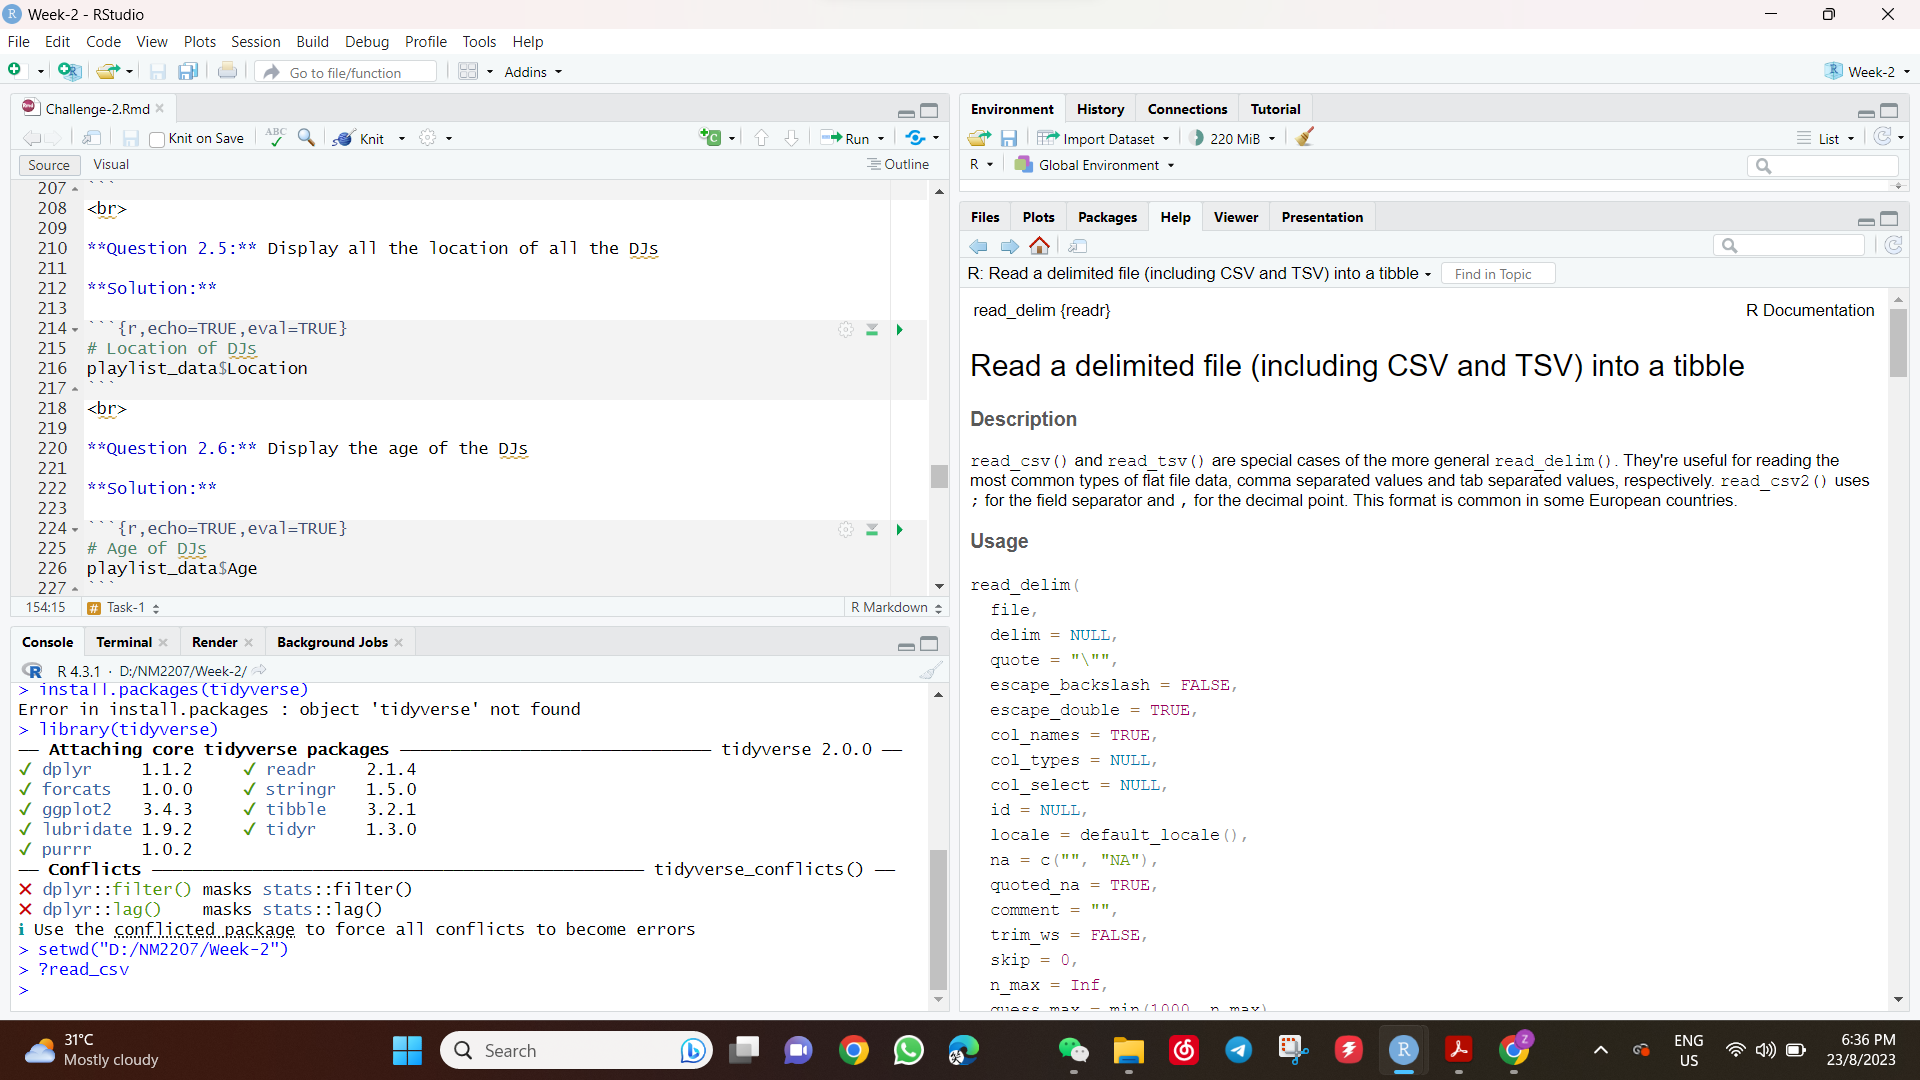
\includegraphics[width=800px,height=400px]{read_csv} \caption{?read_csv}\label{fig:unnamed-chunk-5}
\end{figure}

\textbf{Question 1.6:} What does the \texttt{skip} argument in the
read\_csv() function do?

\textbf{Solution:} Number of lines to skip before reading data. If
comment is supplied any commented lines are ignored after skipping.

\textbf{Question 1.7:} Display the contents of the data-set

\textbf{Solution:}

\begin{Shaded}
\begin{Highlighting}[]
\CommentTok{\# Type the name of the variable, to see what it contains}
\NormalTok{playlist\_data}
\end{Highlighting}
\end{Shaded}

\hypertarget{a-tibble-26-x-7-1}{%
\section{A tibble: 26 x 7}\label{a-tibble-26-x-7-1}}

DJ\_Name Music\_Genre Rating Experience Age Location Plays\_Per\_Week 1
DJ A Pop 4.2 Advanced 28 City X 80 2 DJ B Rock 3.8 Intermediate 24 City
Y 60 3 DJ C Electronic 4.5 Advanced 30 City Z 100 4 DJ D Pop 4
Intermediate 22 City X 70 5 DJ E Electronic 4.8 Advanced 27 City Y 90 6
DJ F Rock 3.6 Intermediate 25 City Z 55 7 DJ G Pop 4.3 Advanced 29 City
X 85 8 DJ H Electronic 4.1 Intermediate 23 City Y 75 9 DJ I Rock 3.9
Advanced 31 City Z 70 10 DJ J Pop 4.4 Intermediate 26 City X 95 \# i 16
more rows

\textbf{Question 1.8:} Assume you have a CSV file named
\(`sales_data.csv`\) containing information about sales transactions.
How would you use the \(`read_csv()`\) function to import this file into
R and store it in a variable named \(`sales_data`\)?

\textbf{Solution:}

\begin{Shaded}
\begin{Highlighting}[]
\CommentTok{\# No output is required for this code}
\CommentTok{\# Only the list of commands that execute the task mentioned in the question are required}
\NormalTok{sales\_data }\OtherTok{\textless{}{-}} \FunctionTok{read\_csv}\NormalTok{(}\StringTok{"sales\_data.csv"}\NormalTok{)}
\end{Highlighting}
\end{Shaded}

\hypertarget{task-2}{%
\paragraph{Task-2}\label{task-2}}

After learning to import a data-set, let us explore the contents of the
data-set through the following questions

\textbf{Question 2.1:} Display the first few rows of the data-set to get
an overview of its structure

\textbf{Solution:}

\begin{Shaded}
\begin{Highlighting}[]
\CommentTok{\# Type the name of the variable we assigned the data{-}set to}
\FunctionTok{head}\NormalTok{(playlist\_data)}
\end{Highlighting}
\end{Shaded}

\hypertarget{a-tibble-6-x-7}{%
\section{A tibble: 6 x 7}\label{a-tibble-6-x-7}}

DJ\_Name Music\_Genre Rating Experience Age Location Plays\_Per\_Week 1
DJ A Pop 4.2 Advanced 28 City X 80 2 DJ B Rock 3.8 Intermediate 24 City
Y 60 3 DJ C Electronic 4.5 Advanced 30 City Z 100 4 DJ D Pop 4
Intermediate 22 City X 70 5 DJ E Electronic 4.8 Advanced 27 City Y 90 6
DJ F Rock 3.6 Intermediate 25 City Z 55

\textbf{Question 2.2:} Display all the columns of the variable stacked
one below another

\textbf{Solution:}

\begin{Shaded}
\begin{Highlighting}[]
\CommentTok{\# Stack columns of playlist\_data}
\FunctionTok{glimpse}\NormalTok{(playlist\_data)}
\end{Highlighting}
\end{Shaded}

Rows: 26 Columns: 7 \$ DJ\_Name ``DJ A'', ``DJ B'', ``DJ C'', ``DJ D'',
``DJ E'', ``DJ F'', ``DJ G'',\textasciitilde{} \$ Music\_Genre ``Pop'',
``Rock'', ``Electronic'', ``Pop'', ``Electronic'',
``Rock\textasciitilde{} \$ Rating 4.2, 3.8, 4.5, 4.0, 4.8, 3.6, 4.3,
4.1, 3.9, 4.4, 4.6, \textasciitilde{} \$ Experience ''Advanced'',
``Intermediate'', ``Advanced'', ``Intermediate'',\textasciitilde{} \$
Age 28, 24, 30, 22, 27, 25, 29, 23, 31, 26, 32, 28, 29,
25,\textasciitilde{} \$ Location ``City X'', ``City Y'', ``City Z'',
``City X'', ``City Y'', ``City\textasciitilde{} \$ Plays\_Per\_Week 80,
60, 100, 70, 90, 55, 85, 75, 70, 95, 110, 75, 60, 8\textasciitilde{}

\begin{Shaded}
\begin{Highlighting}[]
\FunctionTok{str}\NormalTok{(playlist\_data)}
\end{Highlighting}
\end{Shaded}

spc\_tbl\_ {[}26 x 7{]} (S3: spec\_tbl\_df/tbl\_df/tbl/data.frame) \$
DJ\_Name : chr {[}1:26{]} ``DJ A'' ``DJ B'' ``DJ C'' ``DJ D'' \ldots{}
\$ Music\_Genre : chr {[}1:26{]} ``Pop'' ``Rock'' ``Electronic'' ``Pop''
\ldots{} \$ Rating : num {[}1:26{]} 4.2 3.8 4.5 4 4.8 3.6 4.3 4.1 3.9
4.4 \ldots{} \$ Experience : chr {[}1:26{]} ``Advanced''
``Intermediate'' ``Advanced'' ``Intermediate'' \ldots{} \$ Age : num
{[}1:26{]} 28 24 30 22 27 25 29 23 31 26 \ldots{} \$ Location : chr
{[}1:26{]} ``City X'' ``City Y'' ``City Z'' ``City X'' \ldots{} \$
Plays\_Per\_Week: num {[}1:26{]} 80 60 100 70 90 55 85 75 70 95 \ldots{}
- attr(\emph{, ``spec'')= .. cols( .. DJ\_Name = col\_character(), ..
Music\_Genre = col\_character(), .. Rating = col\_double(), ..
Experience = col\_character(), .. Age = col\_double(), .. Location =
col\_character(), .. Plays\_Per\_Week = col\_double() .. ) - attr(},
``problems'')=

\textbf{Question 2.3:} How many columns are there in the dataset?

\textbf{Solution:}

\begin{Shaded}
\begin{Highlighting}[]
\CommentTok{\# Number of columns}
\FunctionTok{ncol}\NormalTok{(playlist\_data)}
\end{Highlighting}
\end{Shaded}

{[}1{]} 7

\textbf{Question 2.4:} What is the total count of DJs?

\textbf{Solution:}

\begin{Shaded}
\begin{Highlighting}[]
\CommentTok{\# Number of DJs}
\FunctionTok{nrow}\NormalTok{(playlist\_data)}
\end{Highlighting}
\end{Shaded}

{[}1{]} 26

\textbf{Question 2.5:} Display all the location of all the DJs

\textbf{Solution:}

\begin{Shaded}
\begin{Highlighting}[]
\CommentTok{\# Location of DJs}
\NormalTok{playlist\_data}\SpecialCharTok{$}\NormalTok{Location}
\end{Highlighting}
\end{Shaded}

{[}1{]} ``City X'' ``City Y'' ``City Z'' ``City X'' ``City Y'' ``City
Z'' ``City X'' ``City Y'' {[}9{]} ``City Z'' ``City X'' ``City Y''
``City Z'' ``City X'' ``City Y'' ``City Z'' ``City X'' {[}17{]} ``City
Y'' ``City Z'' ``City X'' ``City Y'' ``City Z'' ``City X'' ``City Y''
``City Z'' {[}25{]} ``City X'' ``City Y''

\textbf{Question 2.6:} Display the age of the DJs

\textbf{Solution:}

\begin{Shaded}
\begin{Highlighting}[]
\CommentTok{\# Age of DJs}
\NormalTok{playlist\_data}\SpecialCharTok{$}\NormalTok{Age}
\end{Highlighting}
\end{Shaded}

{[}1{]} 28 24 30 22 27 25 29 23 31 26 32 28 29 25 31 26 27 24 29 23 28
24 30 22 27 {[}26{]} 25

\hypertarget{task-3}{%
\paragraph{Task-3}\label{task-3}}

Let us plot the data to get more insights about the DJs.

\textbf{Question 3.1:} Create a plot to visualize the relationship
between DJs' ages and their ratings.

\textbf{Solution:}

\begin{Shaded}
\begin{Highlighting}[]
\CommentTok{\# complete the code to generate the plot}

\FunctionTok{ggplot}\NormalTok{(playlist\_data)}
\end{Highlighting}
\end{Shaded}

\includegraphics{Challenge-2_files/figure-latex/unnamed-chunk-14-1.pdf}

\textbf{Question 3.2:} Label the x-axis as ``Age'' and the y-axis as
``Rating.''

\textbf{Solution:}

\begin{Shaded}
\begin{Highlighting}[]
\CommentTok{\# complete the code to generate the plot}

\FunctionTok{ggplot}\NormalTok{(playlist\_data) }\SpecialCharTok{+} \FunctionTok{aes}\NormalTok{(}\AttributeTok{x=}\NormalTok{Age,}\AttributeTok{y=}\NormalTok{Rating)}
\end{Highlighting}
\end{Shaded}

\includegraphics{Challenge-2_files/figure-latex/unnamed-chunk-15-1.pdf}

\textbf{Question 3.3:} Represent data using points

\textbf{Solution:}

\begin{Shaded}
\begin{Highlighting}[]
\CommentTok{\# complete the code to generate the plot}

\FunctionTok{ggplot}\NormalTok{(playlist\_data) }\SpecialCharTok{+} \FunctionTok{aes}\NormalTok{(}\AttributeTok{x=}\NormalTok{Age,}\AttributeTok{y=}\NormalTok{Rating) }\SpecialCharTok{+} \FunctionTok{geom\_point}\NormalTok{()}
\end{Highlighting}
\end{Shaded}

\includegraphics{Challenge-2_files/figure-latex/unnamed-chunk-16-1.pdf}

\textbf{Question 3.4:} Can you change the points represented by
dots/small circles to any other shape of your liking?

\textbf{Solution:}

\begin{Shaded}
\begin{Highlighting}[]
\CommentTok{\# complete the code to generate the plot}

\FunctionTok{ggplot}\NormalTok{(playlist\_data) }\SpecialCharTok{+} \FunctionTok{aes}\NormalTok{(}\AttributeTok{x=}\NormalTok{Age, }\AttributeTok{y=}\NormalTok{Rating) }\SpecialCharTok{+} \FunctionTok{geom\_point}\NormalTok{(}\AttributeTok{shape =} \DecValTok{17}\NormalTok{, }\AttributeTok{size =} \DecValTok{5}\NormalTok{, }\AttributeTok{colour =} \StringTok{"red"}\NormalTok{)}
\end{Highlighting}
\end{Shaded}

\includegraphics{Challenge-2_files/figure-latex/unnamed-chunk-17-1.pdf}

\begin{Shaded}
\begin{Highlighting}[]
\FunctionTok{geom\_point}\NormalTok{( ) }\CommentTok{\# \textless{}{-}{-} Hint: Use ? to learn more about geom\_point and use appropriate values for shape}
\end{Highlighting}
\end{Shaded}

geom\_point: na.rm = FALSE stat\_identity: na.rm = FALSE
position\_identity

\textbf{Question 3.5:} Insert a suitable title and briefly provide your
insights in the caption

\textbf{Solution:}

\begin{Shaded}
\begin{Highlighting}[]
\CommentTok{\# complete the code to generate the plot}

\FunctionTok{ggplot}\NormalTok{(playlist\_data) }\SpecialCharTok{+} \FunctionTok{aes}\NormalTok{(}\AttributeTok{x=}\NormalTok{Age, }\AttributeTok{y=}\NormalTok{Rating) }\SpecialCharTok{+} \FunctionTok{geom\_point}\NormalTok{(}\AttributeTok{shape =} \DecValTok{17}\NormalTok{, }\AttributeTok{size =} \DecValTok{5}\NormalTok{, }\AttributeTok{colour =} \StringTok{"red"}\NormalTok{) }\SpecialCharTok{+}
\FunctionTok{labs}\NormalTok{(}\AttributeTok{title=}\StringTok{"Rating versus Age"}\NormalTok{, }\AttributeTok{caption =} \StringTok{"Rating and Age are independent of each other."}\NormalTok{)}
\end{Highlighting}
\end{Shaded}

\includegraphics{Challenge-2_files/figure-latex/unnamed-chunk-18-1.pdf}

\end{document}
